\documentclass[UTF8]{ctexart}

\usepackage[colorlinks, urlcolor = blue]{hyperref}
\usepackage{titlesec}
\usepackage{fancyhdr}
\usepackage{tikz}
\usepackage{amssymb}
\usetikzlibrary{shapes.geometric}
\usetikzlibrary{calc}

\title{关于 \LaTeX 文档中 star point ratio 的说明}
\author{}
\date{\today}

\titleformat{\section}{\Large\bf\flushleft}{\thesection}{1em}{}
\setlength{\headheight}{15pt}
\pagestyle{fancy}

\def\rdouter{2}
\def\spratio{cos(36) + sin(36)/tan(18)}
\def\rdinner{\rdouter/(\spratio)}
\newcommand{\tikzprint}{Ti\emph{k}z}

\begin{document}

\maketitle

\section{什么是 star point ratio ?}
根据 \href{http://tug.org/svn/texlive/trunk/Master/texmf-dist/doc/%
generic/pgf/pgfmanual.pdf?revision=51817&view=co}
{\tikzprint~\& PGF Manual for Version 3.1.4b} 中第 781 页的介绍,
star point ratio 是指 outer point 与 inner point 的半径之比。
当通过指定 minimum size 来放大 star 时,
inner point 的半径按此比例随之增大。

这里的 inner point 是指 star 内圈上张角向外的点,
outer point 是指 star 外圈上张角向内的点。
而 star 则是指由若干对内凹(inter point)和外凸(outer point)的点
组成的类似五角星的几何形状。

通俗地说,通过设置 star point ratio 的值,
我们可以控制 star 的“肥瘦”。
当 star point ratio = 1 ,
star points 趋于无穷时,
即为圆。

\begin{center}
  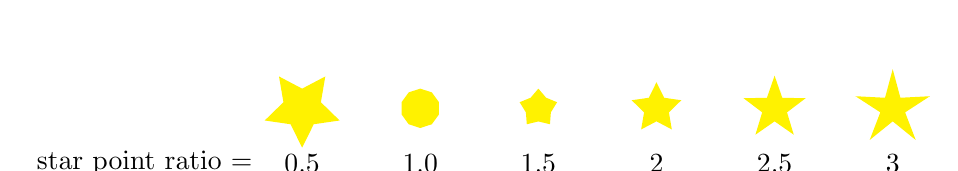
\begin{tikzpicture} 
    \foreach \i in {0.5, 1.0, ..., 3.0} {
      \node[star, fill = yellow, star point ratio = \i,
            minimum size = 0.5 cm]
        at (\i*3, 0) {};
      \node at (\i*3, - 0.7) {\i};
    }
    \node at (- 0.5, - 0.7) {star point ratio =};
  \end{tikzpicture}
\end{center}

\section{为什么是 \spratio ?}
\begin{center}
  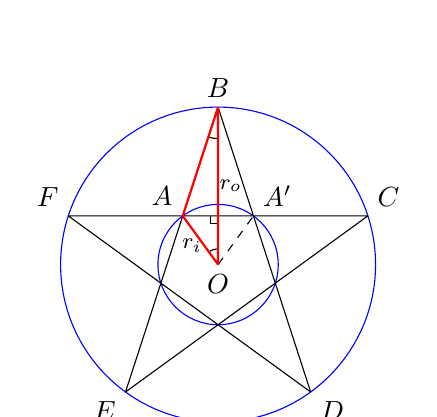
\begin{tikzpicture} [x = 1 cm, y = 1 cm]
    \coordinate (o) at (0, 0);
    \coordinate (a) at ({90 + 36}:{\rdinner});
    \coordinate (b) at (90:{\rdouter});
    \coordinate (c) at ({90 - 360/5*1}:{\rdouter});
    \coordinate (d) at ({90 - 360/5*2}:{\rdouter});
    \coordinate (e) at ({90 - 360/5*3}:{\rdouter});
    \coordinate (f) at ({90 - 360/5*4}:{\rdouter});
    \coordinate (a') at ({90 - 36}:{\rdinner});

    \draw[blue] (o) circle (\rdouter);
    \draw[blue] (o) circle (\rdinner);

    \draw[line join = bevel]
         (b) node[above] {$B$}
      -- (d) node[below right] {$D$}
      -- (f) node[above left] {$F$}
      -- (c) node[above right] {$C$}
      -- (e) node[below left] {$E$}
      -- cycle;
    \draw[dashed, thin] (o) -- (a') node[above right] {$A'$};

    \draw[thin] (o) +(90:0.2) arc (90:{90 + 36}:0.2);
    \draw[thin] (b) +(270:0.4) arc (270:{270 - 18}:0.4);
    \draw[thin] ($(a)!0.5!(a')$) +(180:0.1) |- +(- 90:0.1);

    \draw[thick, red, line join = bevel]
         (o) node[below, black] {$O$}
      -- (a) node[above left, black] {$A$}
      -- (b) -- cycle;
    \draw ($(o)!0.5!(a)$) node[below = 2 pt, left = - 4 pt]
      {\footnotesize $r_i$};
    \draw ($(o)!0.5!(b)$) node[right = - 3 pt]
      {\footnotesize $r_o$};
  \end{tikzpicture}
\end{center}

根据多边形内角和定理可知,
五边形的内角和为 $180^\circ \times (5 - 2) = 540^\circ$,
则 $\angle EAC = 540^\circ \div 5 = 108^\circ$,
$\angle ABA' = \angle ACE = (180^\circ - \angle EAC) \div 2 = 36^\circ$,
$\angle ABO = \angle ABA' \div 2 = 18^\circ$。
而 $\angle AOB = \angle AOA' \div 2 = (360^\circ \div 5) \div 2 = 36^\circ$,
当取 $r_i = \overline{OA} = 1$ 时,则
\[ r_o = \overline{OB} = \cos \angle AOB + \frac{\sin \angle AOB}{\tan \angle ABO}
       = \cos(36^\circ) + \frac{\sin(36^\circ)}{\tan(18^\circ)} \]
此即所谓 star point ratio 。

在 \tikzprint 中,三角函数默认采用角度值进行计算,
因此设置 star point ratio = \spratio 。

\end{document}
